\documentclass[aspectratio=169]{beamer}
\usepackage[utf8]{inputenc}
\usepackage{lmodern}
\usepackage{tikz}
\usepackage{hyperref}
\usetikzlibrary{positioning,arrows.meta,calc}

\definecolor{accent1}{HTML}{7C3AED}
\definecolor{accent2}{HTML}{C4B5FD}
\definecolor{accent3}{HTML}{F472B6}
\definecolor{accent4}{HTML}{312E81}
\definecolor{paper}{HTML}{FCFAFF}
\definecolor{ink}{HTML}{1F2937}

\setbeamertemplate{navigation symbols}{}
\setbeamercolor{normal text}{fg=ink,bg=white}
\setbeamercolor{frametitle}{fg=ink,bg=white}
\setbeamertemplate{itemize item}{\color{accent1}$\blacktriangleright$}
\setbeamertemplate{enumerate item}{\color{accent1}\insertenumlabel.}
\setbeameroption{hide notes}

\title{Google Slides Monopoly | (Day 2)}
\subtitle{Student Guide}
\author{Pine Brook IGNITE}
\date{Spring 2026}

\begin{document}

\begin{frame}[plain]
\begin{tikzpicture}[remember picture,overlay]
\fill[paper] (current page.south west) rectangle (current page.north east);
\fill[accent1!10] (0.25,0.4) rectangle (13.05,7.0);
\draw[line width=7pt, color=accent3] (0.55,6.75) -- (12.75,6.75);
\draw[line width=7pt, color=accent2] (0.55,0.65) -- (12.75,0.65);
\end{tikzpicture}
\vspace{0.45cm}
\begin{columns}[T,totalwidth=\textwidth]
\column{0.56\textwidth}
{\huge\bfseries\color{ink} Google Slides Monopoly | (Day 2)\par}
\vspace{0.2cm}
{\Large\color{accent4} Create. Add. Share.\par}
\vspace{0.25cm}
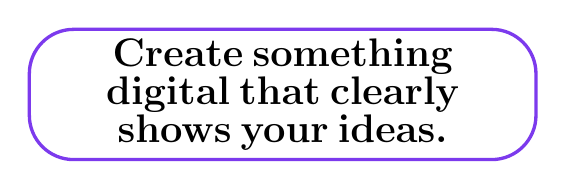
\begin{tikzpicture}
\node[rounded corners=16pt, fill=white, draw=accent1, line width=1.2pt, text width=6.2cm, minimum height=1.35cm, align=center]
{\Large\bfseries Create something digital that clearly shows your ideas.};
\end{tikzpicture}
\vspace{0.35cm}
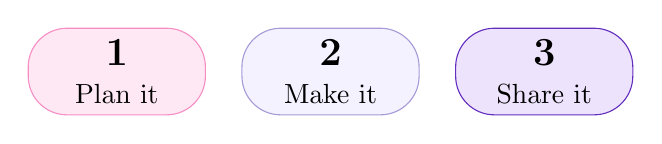
\begin{tikzpicture}[node distance=0.45cm]
\node[rounded corners=14pt, fill=accent3!16, draw=accent3!80, minimum width=2.25cm, minimum height=1.1cm, align=center] (a) {\Large\bfseries 1\\[2pt]Plan it};
\node[rounded corners=14pt, fill=accent2!18, draw=accent2!85!black, minimum width=2.25cm, minimum height=1.1cm, align=center, right=of a] (b) {\Large\bfseries 2\\[2pt]Make it};
\node[rounded corners=14pt, fill=accent1!14, draw=accent1!80!black, minimum width=2.25cm, minimum height=1.1cm, align=center, right=of b] (c) {\Large\bfseries 3\\[2pt]Share it};
\end{tikzpicture}
\column{0.4\textwidth}
\begin{center}

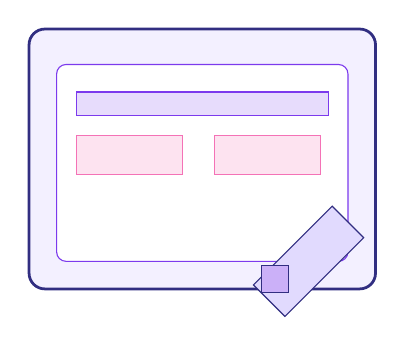
\begin{tikzpicture}[x=1cm,y=1cm]
\draw[rounded corners=0.2cm, fill=accent2!20, draw=accent4, line width=1pt] (0.4,0.5) rectangle (4.8,3.8);
\draw[rounded corners=0.12cm, fill=white, draw=accent1] (0.75,0.85) rectangle (4.45,3.35);
\draw[fill=accent1!18, draw=accent1] (1.0,2.7) rectangle (4.2,3.0);
\draw[fill=accent3!20, draw=accent3] (1.0,1.95) rectangle (2.35,2.45);
\draw[fill=accent3!20, draw=accent3] (2.75,1.95) rectangle (4.1,2.45);
\draw[fill=accent2!50, draw=accent4] (3.65,0.15) -- (4.65,1.15) -- (4.25,1.55) -- (3.25,0.55) -- cycle;
\draw[fill=accent1!40, draw=accent4] (3.35,0.45) rectangle (3.7,0.8);
\end{tikzpicture}

\end{center}
\end{columns}
\note{Audience guidance: Growing independent learners who can handle more tool variety when routines and choices stay well scaffolded.. Teaching move: Model the first screen and the exact tool students must use before release.}
\end{frame}

\begin{frame}[plain]
\frametitle{Today's Mission}
\begin{columns}[T,totalwidth=\textwidth]
\column{0.56\textwidth}
\begin{block}{Our focus}
\normalsize Create something digital and make your ideas clear.
\end{block}
\vspace{0.1cm}
\begin{itemize}
\large
\item I can finish my work.
\item I can show one smart choice I made.
\item I can share my work with a screenshot, demo, or quick talk.
\end{itemize}
\column{0.38\textwidth}
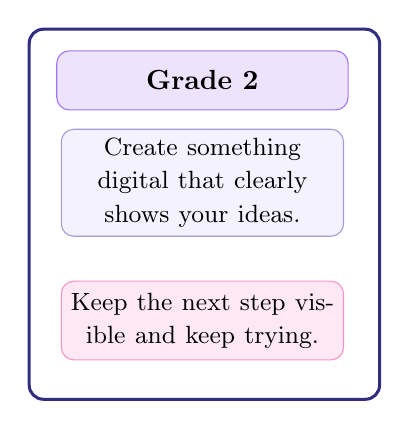
\begin{tikzpicture}[x=1cm,y=1cm]
\draw[rounded corners=0.18cm, fill=white, draw=accent4, line width=1.1pt] (0.1,0.1) rectangle (4.55,4.8);
\node[rounded corners=0.16cm, fill=accent1!14, draw=accent1!70, minimum width=3.7cm, minimum height=0.75cm, align=center] at (2.3,4.15) {\bfseries Grade 2};
\node[rounded corners=0.16cm, fill=accent2!18, draw=accent2!85!black, text width=3.35cm, minimum height=1.2cm, align=center] at (2.3,2.85) {\small Create something digital that clearly shows your ideas.};
\node[rounded corners=0.16cm, fill=accent3!16, draw=accent3!75, text width=3.35cm, minimum height=1.0cm, align=center] at (2.3,1.1) {\small Keep the next step visible and keep trying.};
\end{tikzpicture}
\end{columns}
\note{Open with the mission in student language. Keep the focus visible while students work.} 
\end{frame}

\begin{frame}[plain]
\frametitle{How We Will Move Through It}
\begin{center}
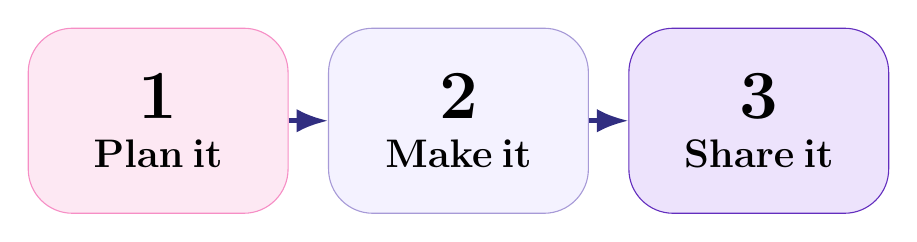
\begin{tikzpicture}[node distance=0.5cm]
\node[rounded corners=16pt, fill=accent3!16, draw=accent3!80, minimum width=3.3cm, minimum height=2.35cm, text width=2.45cm, align=center] (s1) {\Huge\bfseries 1\\[6pt]\Large Plan it};
\node[rounded corners=16pt, fill=accent2!18, draw=accent2!85!black, minimum width=3.3cm, minimum height=2.35cm, text width=2.45cm, align=center, right=of s1] (s2) {\Huge\bfseries 2\\[6pt]\Large Make it};
\node[rounded corners=16pt, fill=accent1!14, draw=accent1!80!black, minimum width=3.3cm, minimum height=2.35cm, text width=2.45cm, align=center, right=of s2] (s3) {\Huge\bfseries 3\\[6pt]\Large Share it};
\draw[-{Latex[length=4mm,width=3mm]}, line width=1.7pt, color=accent4] (s1) -- (s2);
\draw[-{Latex[length=4mm,width=3mm]}, line width=1.7pt, color=accent4] (s2) -- (s3);
\end{tikzpicture}
\end{center}
\vspace{0.25cm}
\begin{block}{What to keep in front of you}
\begin{itemize}
\large
\item Watch the first step.
\item Use the checklist or example.
\item Pause, check, and keep going.
\end{itemize}
\end{block}
\note{Keep this slide up during work time when students need a visible routine.} 
\end{frame}

\begin{frame}[plain]
\frametitle{If You Get Stuck}
\begin{columns}[T,totalwidth=\textwidth]
\column{0.5\textwidth}
\begin{block}{Use this help ladder}
\begin{enumerate}
\large
\item Look at the slide.
\item Try one small step.
\item Ask your partner.
\item Ask one clear question.
\end{enumerate}
\end{block}
\column{0.45\textwidth}
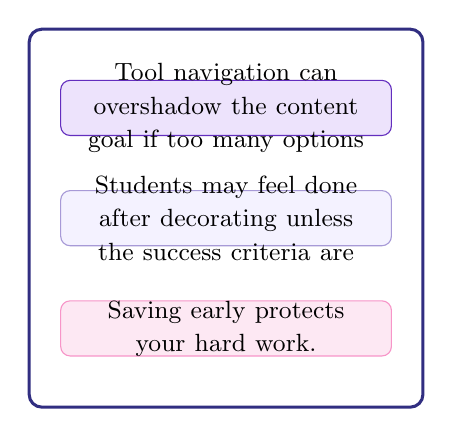
\begin{tikzpicture}[x=1cm,y=1cm]
\draw[rounded corners=0.16cm, fill=white, draw=accent4, line width=1.1pt] (0.0,0.0) rectangle (5.0,4.8);
\draw[rounded corners=0.12cm, fill=accent1!14, draw=accent1!80!black] (0.4,3.45) rectangle (4.6,4.15);
\node[text width=3.7cm, align=center] at (2.5,3.8) {\small Tool navigation can overshadow the content goal if too many options};
\draw[rounded corners=0.12cm, fill=accent2!18, draw=accent2!85!black] (0.4,2.05) rectangle (4.6,2.75);
\node[text width=3.7cm, align=center] at (2.5,2.4) {\small Students may feel done after decorating unless the success criteria are};
\draw[rounded corners=0.12cm, fill=accent3!16, draw=accent3!75] (0.4,0.65) rectangle (4.6,1.35);
\node[text width=3.7cm, align=center] at (2.5,1.0) {\small Saving early protects your hard work.};
\end{tikzpicture}
\end{columns}
\note{Name the next small move. Hints before rescues.} 
\end{frame}

\begin{frame}[plain]
\frametitle{Show What You Learned}
\begin{center}
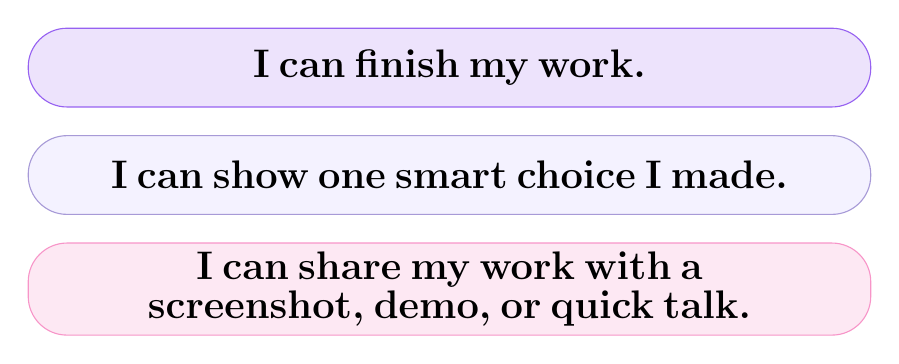
\begin{tikzpicture}[node distance=0.35cm]
\node[rounded corners=14pt, fill=accent1!14, draw=accent1!80, minimum width=10.7cm, minimum height=1.0cm, text width=9.5cm, align=center] (a) {\Large\bfseries I can finish my work.};
\node[rounded corners=14pt, fill=accent2!18, draw=accent2!85!black, minimum width=10.7cm, minimum height=1.0cm, text width=9.5cm, align=center, below=of a] (b) {\Large\bfseries I can show one smart choice I made.};
\node[rounded corners=14pt, fill=accent3!16, draw=accent3!75, minimum width=10.7cm, minimum height=1.0cm, text width=9.5cm, align=center, below=of b] (c) {\Large\bfseries I can share my work with a screenshot, demo, or quick talk.};
\end{tikzpicture}
\end{center}
\vspace{0.28cm}
\begin{block}{Finish strong}
\Large Save it, share it, explain it, or demonstrate it.
\end{block}
\note{Close with one visible proof move and one clear celebration cue.}
\end{frame}

\end{document}
